% Created by tikzDevice version 0.12.3.1 on 2021-11-20 21:14:50
% !TEX encoding = UTF-8 Unicode
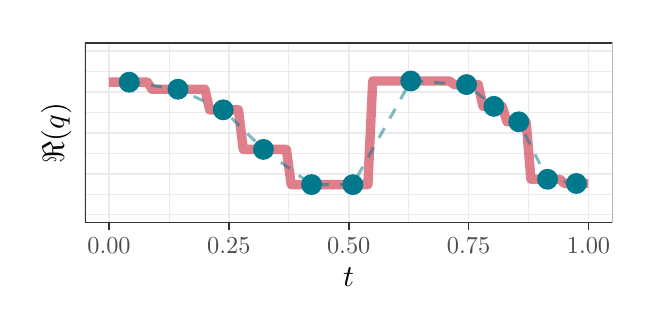
\begin{tikzpicture}[x=1pt,y=1pt]
\definecolor{fillColor}{RGB}{255,255,255}
\path[use as bounding box,fill=fillColor,fill opacity=0.00] (0,0) rectangle (216.81,101.18);
\begin{scope}
\path[clip] (  0.00,  0.00) rectangle (216.81,101.18);
\definecolor{drawColor}{RGB}{255,255,255}
\definecolor{fillColor}{RGB}{255,255,255}

\path[draw=drawColor,line width= 0.6pt,line join=round,line cap=round,fill=fillColor] (  0.00,  0.00) rectangle (216.81,101.18);
\end{scope}
\begin{scope}
\path[clip] ( 20.71, 30.69) rectangle (211.31, 95.68);
\definecolor{fillColor}{RGB}{255,255,255}

\path[fill=fillColor] ( 20.71, 30.69) rectangle (211.31, 95.68);
\definecolor{drawColor}{gray}{0.92}

\path[draw=drawColor,line width= 0.3pt,line join=round] ( 20.71, 41.03) --
	(211.31, 41.03);

\path[draw=drawColor,line width= 0.3pt,line join=round] ( 20.71, 55.80) --
	(211.31, 55.80);

\path[draw=drawColor,line width= 0.3pt,line join=round] ( 20.71, 70.57) --
	(211.31, 70.57);

\path[draw=drawColor,line width= 0.3pt,line join=round] ( 20.71, 85.34) --
	(211.31, 85.34);

\path[draw=drawColor,line width= 0.3pt,line join=round] ( 51.04, 30.69) --
	( 51.04, 95.68);

\path[draw=drawColor,line width= 0.3pt,line join=round] ( 94.35, 30.69) --
	( 94.35, 95.68);

\path[draw=drawColor,line width= 0.3pt,line join=round] (137.67, 30.69) --
	(137.67, 95.68);

\path[draw=drawColor,line width= 0.3pt,line join=round] (180.99, 30.69) --
	(180.99, 95.68);

\path[draw=drawColor,line width= 0.6pt,line join=round] ( 20.71, 33.64) --
	(211.31, 33.64);

\path[draw=drawColor,line width= 0.6pt,line join=round] ( 20.71, 48.41) --
	(211.31, 48.41);

\path[draw=drawColor,line width= 0.6pt,line join=round] ( 20.71, 63.18) --
	(211.31, 63.18);

\path[draw=drawColor,line width= 0.6pt,line join=round] ( 20.71, 77.95) --
	(211.31, 77.95);

\path[draw=drawColor,line width= 0.6pt,line join=round] ( 20.71, 92.72) --
	(211.31, 92.72);

\path[draw=drawColor,line width= 0.6pt,line join=round] ( 29.38, 30.69) --
	( 29.38, 95.68);

\path[draw=drawColor,line width= 0.6pt,line join=round] ( 72.69, 30.69) --
	( 72.69, 95.68);

\path[draw=drawColor,line width= 0.6pt,line join=round] (116.01, 30.69) --
	(116.01, 95.68);

\path[draw=drawColor,line width= 0.6pt,line join=round] (159.33, 30.69) --
	(159.33, 95.68);

\path[draw=drawColor,line width= 0.6pt,line join=round] (202.65, 30.69) --
	(202.65, 95.68);
\definecolor{drawColor}{RGB}{209,73,91}

\path[draw=drawColor,draw opacity=0.70,line width= 3.4pt,line join=round] ( 29.38, 81.48) --
	( 31.11, 81.48) --
	( 32.84, 81.48) --
	( 34.58, 81.48) --
	( 36.31, 81.48) --
	( 38.04, 81.48) --
	( 39.77, 81.48) --
	( 41.51, 81.48) --
	( 43.24, 81.48) --
	( 44.97, 78.94) --
	( 46.70, 78.94) --
	( 48.44, 78.94) --
	( 50.17, 78.94) --
	( 51.90, 78.94) --
	( 53.64, 78.94) --
	( 55.37, 78.94) --
	( 57.10, 78.94) --
	( 58.83, 78.94) --
	( 60.57, 78.94) --
	( 62.30, 78.94) --
	( 64.03, 78.94) --
	( 65.76, 71.49) --
	( 67.50, 71.49) --
	( 69.23, 71.49) --
	( 70.96, 71.49) --
	( 72.69, 71.49) --
	( 74.43, 71.49) --
	( 76.16, 71.49) --
	( 77.89, 57.19) --
	( 79.63, 57.19) --
	( 81.36, 57.19) --
	( 83.09, 57.19) --
	( 84.82, 57.19) --
	( 86.56, 57.19) --
	( 88.29, 57.19) --
	( 90.02, 57.19) --
	( 91.75, 57.19) --
	( 93.49, 57.19) --
	( 95.22, 44.48) --
	( 96.95, 44.48) --
	( 98.69, 44.48) --
	(100.42, 44.48) --
	(102.15, 44.48) --
	(103.88, 44.48) --
	(105.62, 44.48) --
	(107.35, 44.48) --
	(109.08, 44.48) --
	(110.81, 44.48) --
	(112.55, 44.46) --
	(114.28, 44.46) --
	(116.01, 44.46) --
	(117.74, 44.46) --
	(119.48, 44.46) --
	(121.21, 44.46) --
	(122.94, 44.46) --
	(124.68, 81.91) --
	(126.41, 81.91) --
	(128.14, 81.91) --
	(129.87, 81.91) --
	(131.61, 81.91) --
	(133.34, 81.91) --
	(135.07, 81.91) --
	(136.80, 81.91) --
	(138.54, 81.91) --
	(140.27, 81.91) --
	(142.00, 81.91) --
	(143.74, 81.91) --
	(145.47, 81.91) --
	(147.20, 81.91) --
	(148.93, 81.91) --
	(150.67, 81.91) --
	(152.40, 81.91) --
	(154.13, 80.62) --
	(155.86, 80.62) --
	(157.60, 80.62) --
	(159.33, 80.62) --
	(161.06, 80.62) --
	(162.79, 80.62) --
	(164.53, 72.75) --
	(166.26, 72.75) --
	(167.99, 72.75) --
	(169.73, 72.75) --
	(171.46, 72.75) --
	(173.19, 67.17) --
	(174.92, 67.17) --
	(176.66, 67.17) --
	(178.39, 67.17) --
	(180.12, 67.17) --
	(181.85, 46.40) --
	(183.59, 46.40) --
	(185.32, 46.40) --
	(187.05, 46.40) --
	(188.79, 46.40) --
	(190.52, 46.40) --
	(192.25, 46.40) --
	(193.98, 44.88) --
	(195.72, 44.88) --
	(197.45, 44.88) --
	(199.18, 44.88) --
	(200.91, 44.88) --
	(202.65, 44.88);
\definecolor{drawColor}{RGB}{0,121,140}

\path[draw=drawColor,draw opacity=0.50,line width= 1.1pt,dash pattern=on 4pt off 4pt ,line join=round] ( 36.68, 81.48) --
	( 54.31, 78.94) --
	( 70.66, 71.49) --
	( 85.20, 57.19) --
	(102.59, 44.48) --
	(117.50, 44.46) --
	(138.42, 81.91) --
	(158.58, 80.62) --
	(168.46, 72.75) --
	(177.46, 67.17) --
	(187.86, 46.40) --
	(198.27, 44.88);
\definecolor{drawColor}{RGB}{0,121,140}
\definecolor{fillColor}{RGB}{0,121,140}

\path[draw=drawColor,line width= 0.4pt,line join=round,line cap=round,fill=fillColor] ( 36.68, 81.48) circle (  3.57);

\path[draw=drawColor,line width= 0.4pt,line join=round,line cap=round,fill=fillColor] ( 54.31, 78.94) circle (  3.57);

\path[draw=drawColor,line width= 0.4pt,line join=round,line cap=round,fill=fillColor] ( 70.66, 71.49) circle (  3.57);

\path[draw=drawColor,line width= 0.4pt,line join=round,line cap=round,fill=fillColor] ( 85.20, 57.19) circle (  3.57);

\path[draw=drawColor,line width= 0.4pt,line join=round,line cap=round,fill=fillColor] (102.59, 44.48) circle (  3.57);

\path[draw=drawColor,line width= 0.4pt,line join=round,line cap=round,fill=fillColor] (117.50, 44.46) circle (  3.57);

\path[draw=drawColor,line width= 0.4pt,line join=round,line cap=round,fill=fillColor] (138.42, 81.91) circle (  3.57);

\path[draw=drawColor,line width= 0.4pt,line join=round,line cap=round,fill=fillColor] (158.58, 80.62) circle (  3.57);

\path[draw=drawColor,line width= 0.4pt,line join=round,line cap=round,fill=fillColor] (168.46, 72.75) circle (  3.57);

\path[draw=drawColor,line width= 0.4pt,line join=round,line cap=round,fill=fillColor] (177.46, 67.17) circle (  3.57);

\path[draw=drawColor,line width= 0.4pt,line join=round,line cap=round,fill=fillColor] (187.86, 46.40) circle (  3.57);

\path[draw=drawColor,line width= 0.4pt,line join=round,line cap=round,fill=fillColor] (198.27, 44.88) circle (  3.57);
\definecolor{drawColor}{gray}{0.20}

\path[draw=drawColor,line width= 0.6pt,line join=round,line cap=round] ( 20.71, 30.69) rectangle (211.31, 95.68);
\end{scope}
\begin{scope}
\path[clip] (  0.00,  0.00) rectangle (216.81,101.18);
\definecolor{drawColor}{gray}{0.20}

\path[draw=drawColor,line width= 0.6pt,line join=round] ( 29.38, 27.94) --
	( 29.38, 30.69);

\path[draw=drawColor,line width= 0.6pt,line join=round] ( 72.69, 27.94) --
	( 72.69, 30.69);

\path[draw=drawColor,line width= 0.6pt,line join=round] (116.01, 27.94) --
	(116.01, 30.69);

\path[draw=drawColor,line width= 0.6pt,line join=round] (159.33, 27.94) --
	(159.33, 30.69);

\path[draw=drawColor,line width= 0.6pt,line join=round] (202.65, 27.94) --
	(202.65, 30.69);
\end{scope}
\begin{scope}
\path[clip] (  0.00,  0.00) rectangle (216.81,101.18);
\definecolor{drawColor}{gray}{0.30}

\node[text=drawColor,anchor=base,inner sep=0pt, outer sep=0pt, scale=  0.88] at ( 29.38, 19.68) {0.00};

\node[text=drawColor,anchor=base,inner sep=0pt, outer sep=0pt, scale=  0.88] at ( 72.69, 19.68) {0.25};

\node[text=drawColor,anchor=base,inner sep=0pt, outer sep=0pt, scale=  0.88] at (116.01, 19.68) {0.50};

\node[text=drawColor,anchor=base,inner sep=0pt, outer sep=0pt, scale=  0.88] at (159.33, 19.68) {0.75};

\node[text=drawColor,anchor=base,inner sep=0pt, outer sep=0pt, scale=  0.88] at (202.65, 19.68) {1.00};
\end{scope}
\begin{scope}
\path[clip] (  0.00,  0.00) rectangle (216.81,101.18);
\definecolor{drawColor}{RGB}{0,0,0}

\node[text=drawColor,anchor=base,inner sep=0pt, outer sep=0pt, scale=  1.10] at (116.01,  7.64) {$t$};
\end{scope}
\begin{scope}
\path[clip] (  0.00,  0.00) rectangle (216.81,101.18);
\definecolor{drawColor}{RGB}{0,0,0}

\node[text=drawColor,rotate= 90.00,anchor=base,inner sep=0pt, outer sep=0pt, scale=  1.10] at ( 13.08, 63.18) {$\Re(q)$};
\end{scope}
\end{tikzpicture}
